\section{Theorie}
\label{sec:Theorie}

\subsection{Energieverteilung und Sättigungsstrom}

In einem Leiter können sich Elektronen nahezu frei bewegen. Um jedoch den Leiter verlassen zu können, müssen sie wie in dem in Abbildung \ref{fig:pot} dargestellten Potentialtopf die Potentialdifferenz $\phi$ überwinden, also eine Austrittsarbeit von $W_.A=\mathrm{e}_.0\phi$, mit der Elementarladung des Elektrons $\mathrm{e}_.0$, leisten. \newline
Die Energieverteilung ist mit der Fermischen Grenzenergie $\zeta$, der Temperatur $T$ und der Boltzmann-Konstante $k_.B$ gegeben durch die Fermi-Diracsche-Verteilungsfunktion
\[
f(E)= \frac{1}{\exp{\left(\frac{E-\zeta}{k_.BT}\right)}-1}\text{,}
\]
deren Verlauf für verschiedenen Temperaturen in Abbildung \ref{fig:fermi} dargestellt ist.
Die Elektronen müssen also mindestens die Energie $E_.0=\zeta + \mathrm{e}_.0\phi\gg k_.BT$ besitzen um das Material zu verlassen, weshalb die Verteilung zu 
\begin{equation}
f(E)\approx\exp{\left(\frac{-\mathrm{e}_.0\phi}{k_.BT}\right)}\label{eq:FDV}
\end{equation}
genähert werden kann. Da die Elektronen den Leiter nur verlassen können, wenn sie mindestens $E_.0$ als kinetische Energie in Normalenrichtung zur Leiteroberfläche $A$ aufweisen, muss für die Sättigungsstromdichte $j_.S$ über alle Elektronen integriert werden, die diese Energie besitzen. Damit ergibt sich für $j_.S$ die Richardson-Gleichung
\[
j_.S(T)=4\pi\frac{\mathrm{e}_.0m_.0k^2_.B}{h^3}T^2\exp{\left(\frac{-\mathrm{e}_.0\phi}{k_.BT}\right)}
\]
und mit $I=j\cdot A$ für den Sättigungsstrom 
\begin{equation}
I_.S = 4\pi A\frac{\mathrm{e}_.0m_.0k^2_.B}{h^3}T^2\exp{\left(\frac{-\mathrm{e}_.0\phi}{k_.BT}\right)}\text{.}
\end{equation}
Das Plancksche Wirkungsquantum $h$ kommt dabei daher, das jeder Energiezustand im Phasenraum ein Volumen von $h^3$ einnimmt.

\begin{figure}
\centering
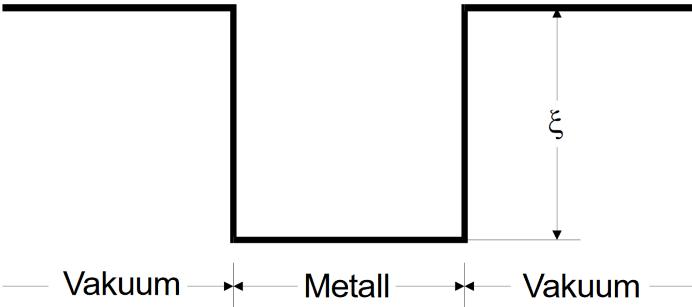
\includegraphics[width=\linewidth-70pt,height=\textheight-70pt,keepaspectratio]{content/images/Pot.jpg}
\caption{Modell eines Potentialtopfs zur Beschreibung der Potentialverhältnisse in einem Leiter\cite{V504}}
\label{fig:pot}
\end{figure}

\begin{figure}
\centering
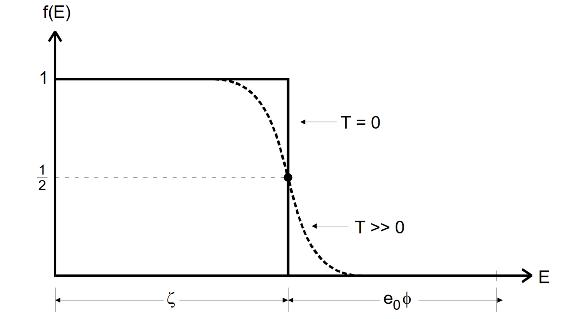
\includegraphics[width=\linewidth-70pt,height=\textheight-70pt,keepaspectratio]{content/images/fermi.jpg}
\caption{Verlauf der Fermi-Dirac-Verteilung am absoluten Nullpunkt und für wesentlich größere Temperaturen\cite{V504}\label{fig:fermi}}
\end{figure}